\documentclass{beamer}
\newcommand \beameritemnestingprefix{}


\usepackage[orientation=landscape,size=a0,scale=1.4,debug]{beamerposter}
\mode<presentation>{\usetheme{mlr}}


\usepackage[utf8]{inputenc} % UTF-8
\usepackage[english]{babel} % Language
\usepackage{hyperref} % Hyperlinks
\usepackage{ragged2e} % Text position
\usepackage[export]{adjustbox} % Image position
\usepackage[most]{tcolorbox}
\usepackage{amsmath}
\usepackage{mathtools}
\usepackage{dsfont}
\usepackage{verbatim}
\usepackage{amsmath}
\usepackage{amsfonts}
\usepackage{csquotes}
\usepackage{multirow}
\usepackage{longtable}
\usepackage[absolute,overlay]{textpos}
\usepackage{psfrag}
\usepackage{algorithm}
\usepackage{algpseudocode}
\usepackage{eqnarray}
\usepackage{arydshln}
\usepackage{tabularx}
\usepackage{placeins}
\usepackage{tikz}
\usepackage{setspace}
\usepackage{colortbl}
\usepackage{mathtools}
\usepackage{wrapfig}
\usepackage{bm}


\input{../../latex-math/basic-math.tex}
\input{../../latex-math/basic-ml.tex}
\input{../../latex-math/ml-lm.tex}


\title{I2ML :\,: CHEAT SHEET} % Package title in header, \, adds thin space between ::
\newcommand{\packagedescription}{ % Package description in header
	The \textbf{I2ML}: Introduction to Machine Learning course offers an introductory and applied overview of "supervised" Machine Learning. It is organized as a digital lecture.
}

\newlength{\columnheight} % Adjust depending on header height
\setlength{\columnheight}{84cm} 

\newtcolorbox{codebox}{%
	sharp corners,
	leftrule=0pt,
	rightrule=0pt,
	toprule=0pt,
	bottomrule=0pt,
	hbox}

\newtcolorbox{codeboxmultiline}[1][]{%
	sharp corners,
	leftrule=0pt,
	rightrule=0pt,
	toprule=0pt,
	bottomrule=0pt,
	#1}

\begin{document}
\begin{frame}[fragile]{}
\begin{columns}
	\begin{column}{.31\textwidth}
		\begin{beamercolorbox}[center]{postercolumn}
			\begin{minipage}{.98\textwidth}
				\parbox[t][\columnheight]{\textwidth}{
					\begin{myblock}{Regression Losses}
						\begin{codebox}
			\textbf{Basic Idea (L2 loss/ squared error):}
						\end{codebox}
						
						\begin{itemize}[$\bullet$]     
						\setlength{\itemindent}{+.3in}
              \item $\Lxy = (y-\fx)^2$ or $\Lxy = 0.5 (y-\fx)^2$
              \item Convex and differentiable.
              \item Tries to reduce large residuals (if residual is twice as large, loss is 4 times as large)      
            \end{itemize}

            \vspace*{1ex}
            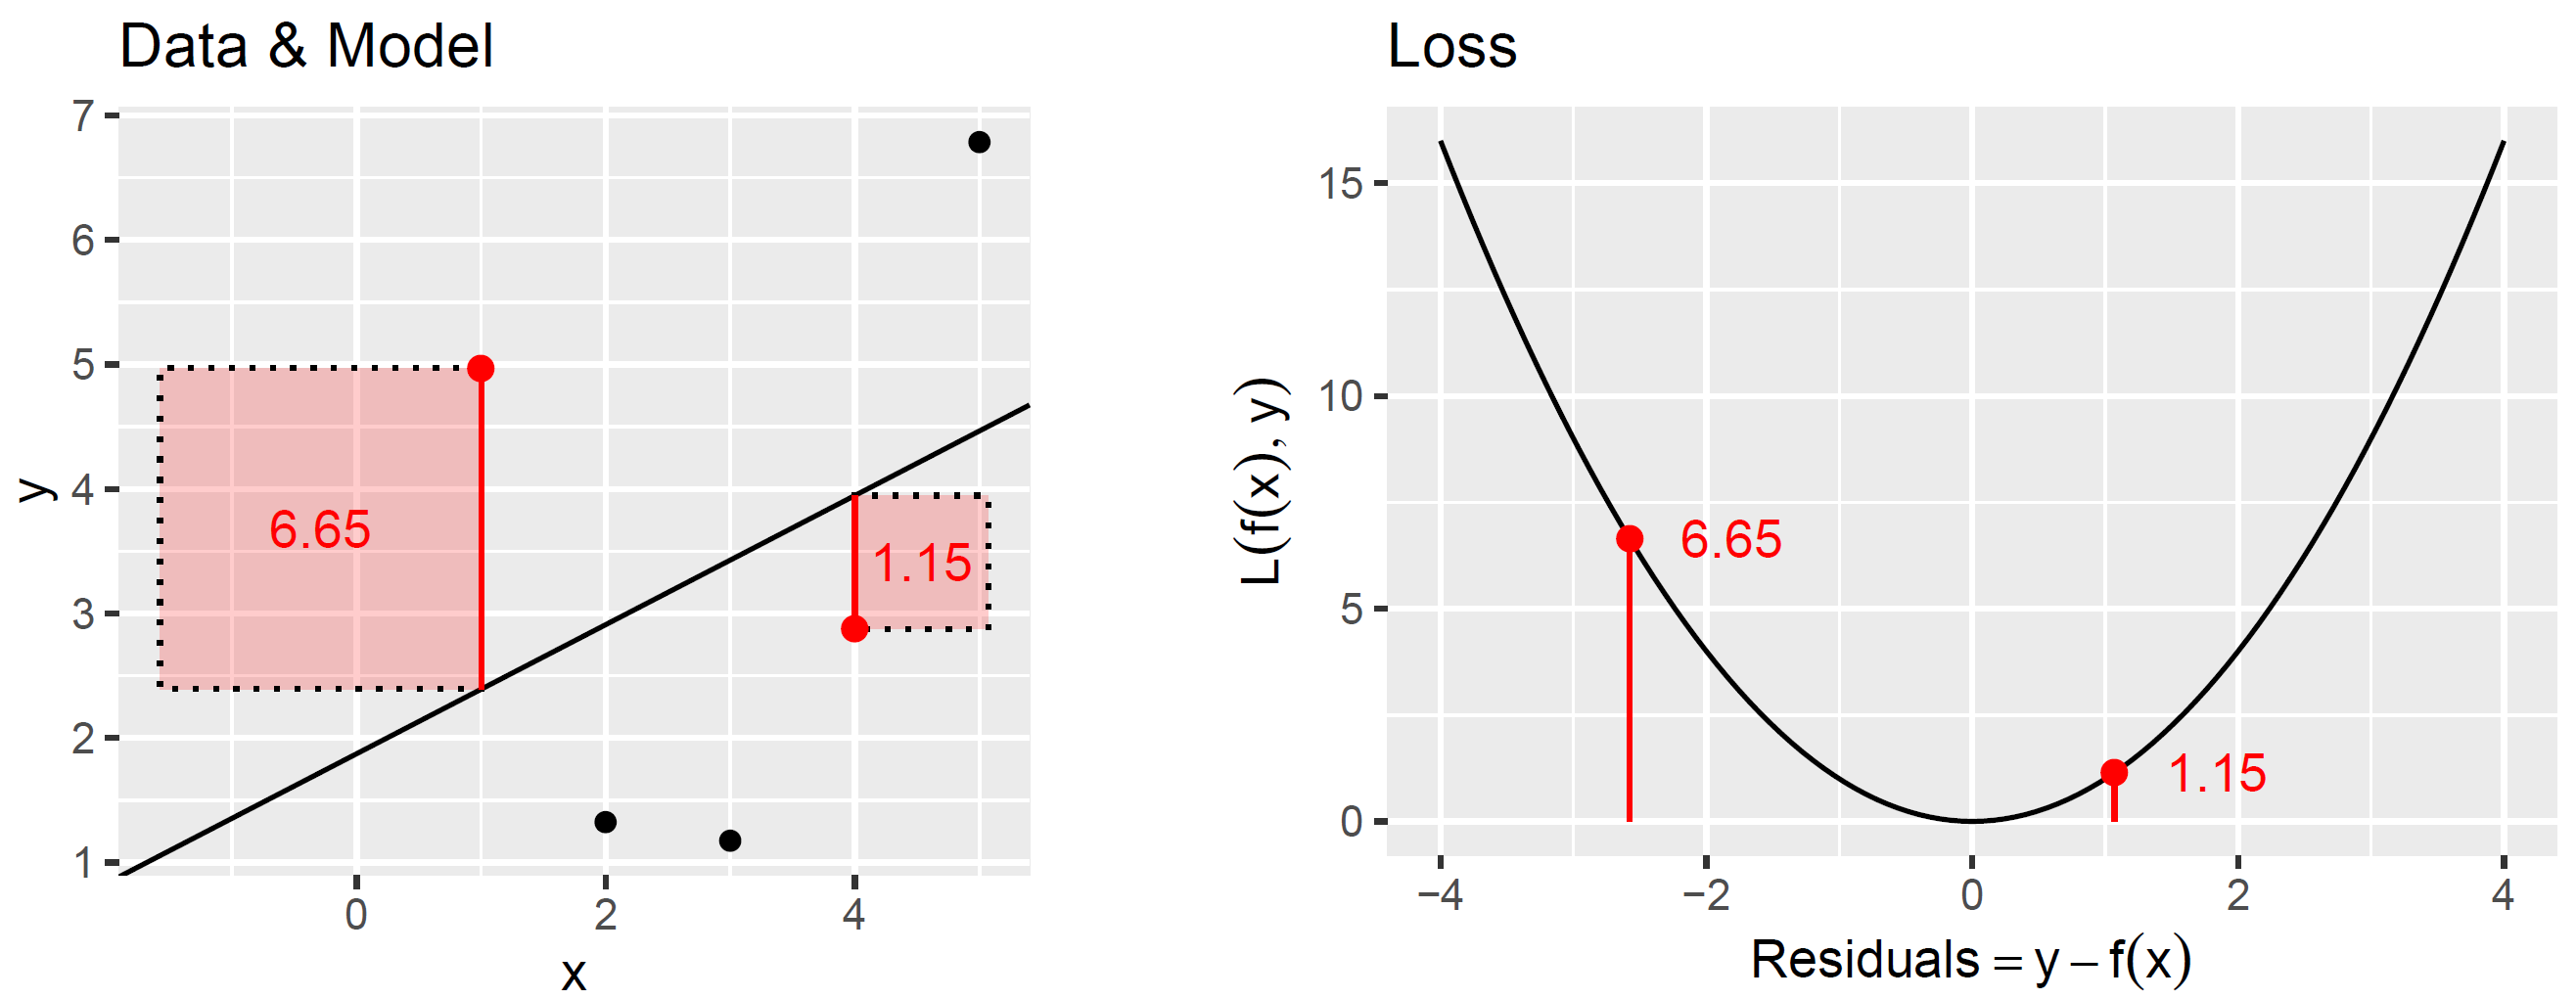
\includegraphics[width=1\columnwidth]{img/reg_loss.PNG}

\begin{codebox}
\textbf{Basic Idea (L1 loss/ absolute error):}
\end{codebox}

\begin{itemize}[$\bullet$]     \setlength{\itemindent}{+.3in}
\item $\Lxy = |y-\fx|$
  \item Convex and more robust
\item No derivatives for $ = 0$, $y = \fx$, optimization becomes harder
\item $\fxh = \text{median of } y | \bm{x}$      
  \end{itemize}

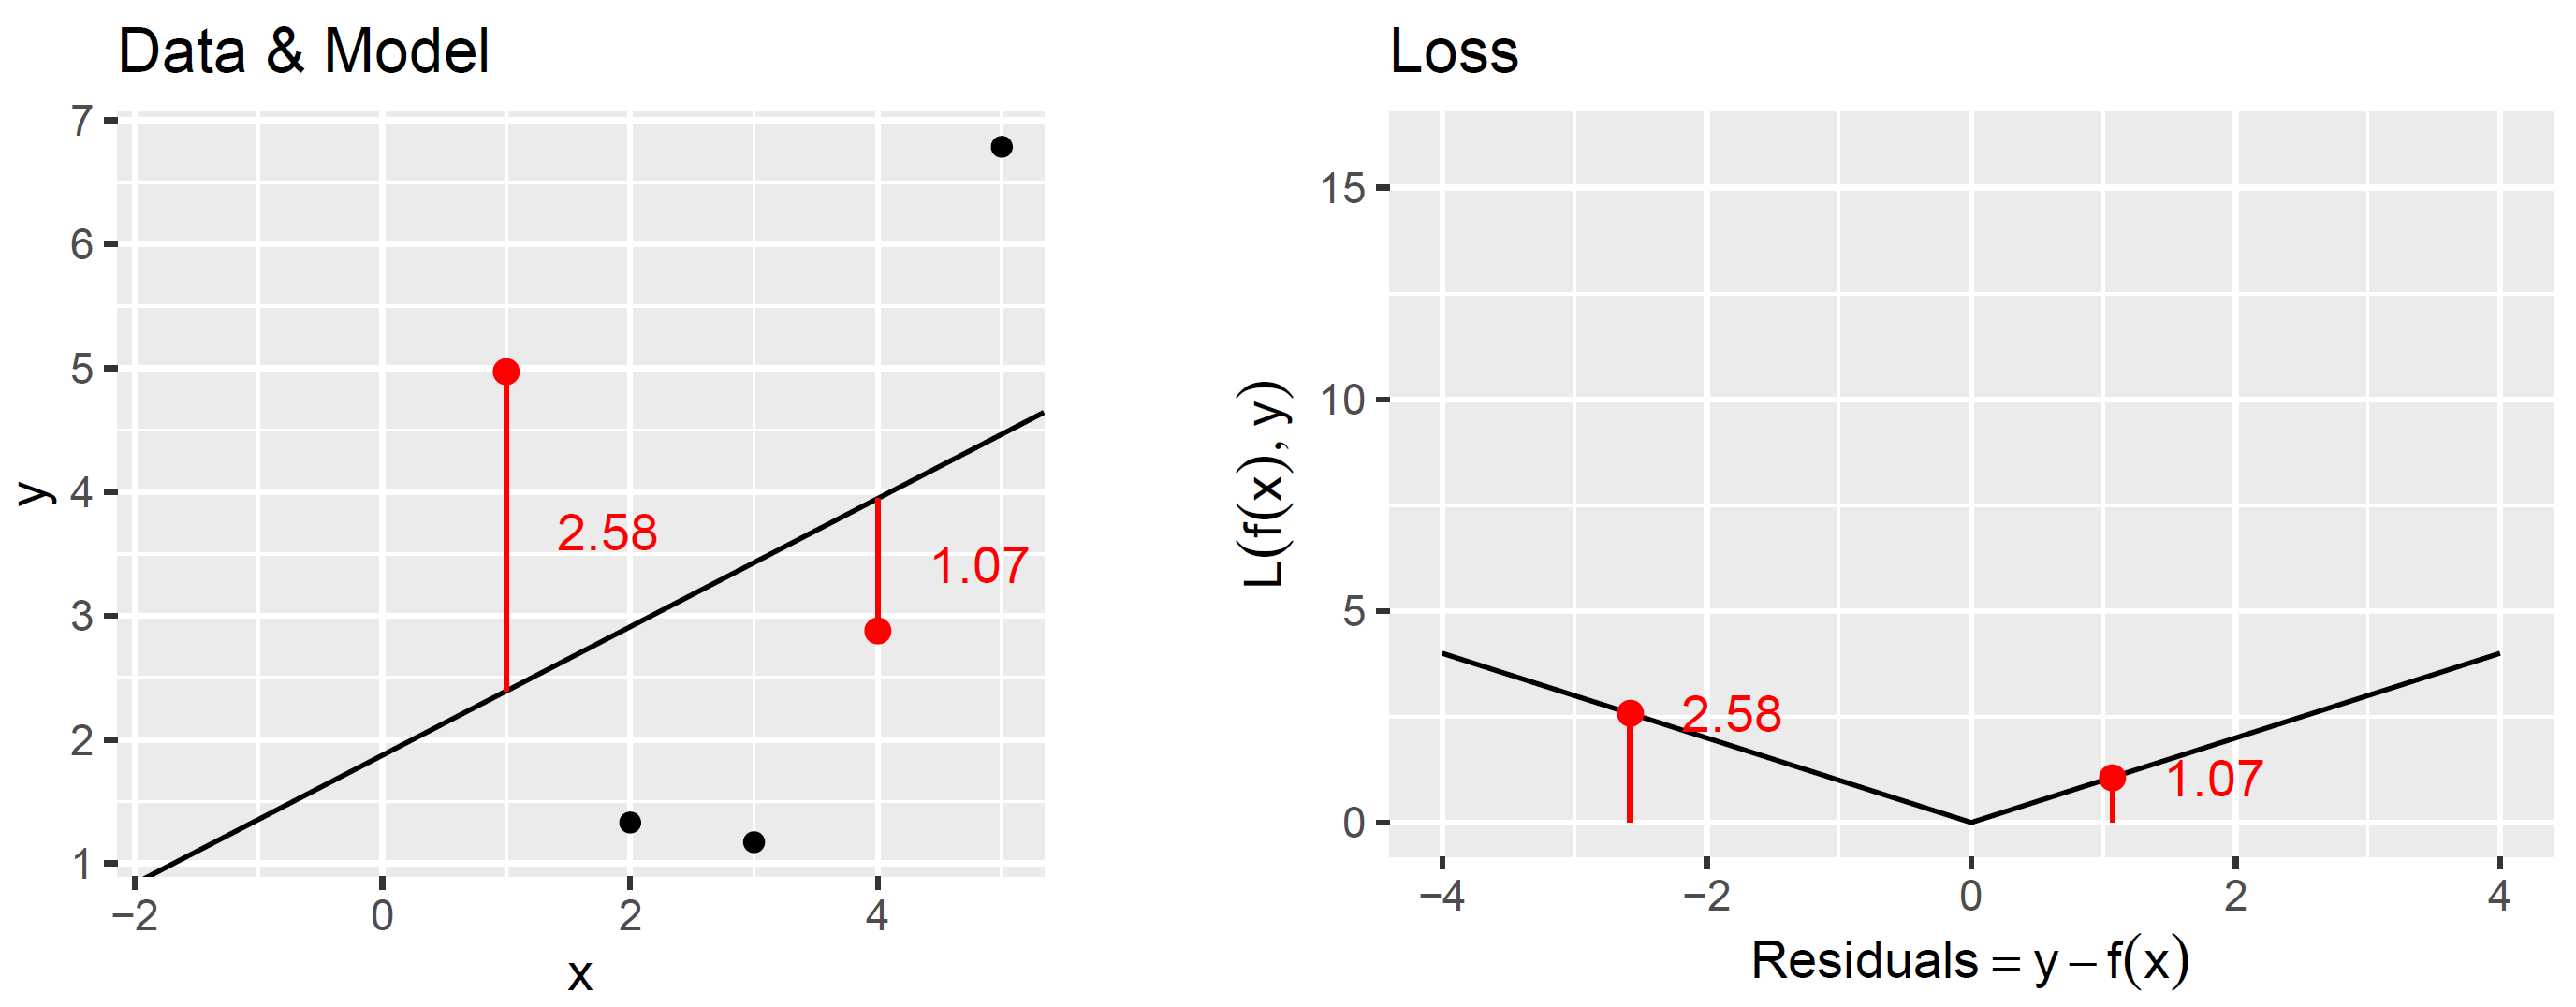
\includegraphics[width=1.03\columnwidth]{img/reg_loss_2.PNG} 

      \end{myblock}
      \begin{myblock}{Linear Regression Models}

\begin{codebox} \textbf{Hypothesis Space: }
\end{codebox}
This defines the hypothesis space $\Hspace$ as the set of all linear functions in $\bm{\theta}$:
\[
  \Hspace = \{ \theta_0 + \thetab^T \xv\ |\ (\theta_0, \thetab) \in \mathbb{R}^{p+1} \}\]
\end{myblock}\vfill
}
			\end{minipage}
		\end{beamercolorbox}
	\end{column}

%%%%%%%%%%%%%%%%%%%%%%%%%%%%%%%%%%%%%%%%%%%%%%%%%%%%%%%%%%%%%%%%%%%%%%%%%%%%%%%%%%%%%%%%%%%%%%%%%%%%%%%%%%%%%%%%%%%%%

\begin{column}{.31\textwidth}
\begin{beamercolorbox}[center]{postercolumn}
\begin{minipage}{.98\textwidth}
\parbox[t][\columnheight]{\textwidth}{
  \begin{myblock}{ }
  \begin{codebox}
  \textbf{Risk (corresponding to \textbf{L2 Loss}):}	\end{codebox} 
  \[\risket = \operatorname{SSE}(\thetab) = \sumin \Lxyit = \sumin \left(\yi - \thetab^T \xi\right)^2\]
  
  \begin{codebox}
  \textbf{Risk (corresponding to \textbf{L1 Loss}):}
  \end{codebox}
  \[
    \risket = \sumin \Lxyit = \sumin \left|\yi - \theta^T \xi\right| \qquad
    \]
  L1 loss is harder to optimize, but the model is less sensitive to outliers
  
  \begin{codebox}
  \textbf{Summary:}
  \end{codebox}
  \textbf{Hypothesis Space:} Linear functions $\xv^T\thetab$ of features $\in \Xspace$.
  
  \vspace*{1ex}
  
  \textbf{Risk:} Any regression loss function.
  
  \vspace*{1ex}
  
  \textbf{Optimization:} Direct analytic solution for L2 loss, numerical optimization for L1 and others.
  \end{myblock}
  
  \begin{myblock}{Polynomial Regression Models}
  
  Linear regression models can be made more flexible by using \emph{polynomials} $x_j^d$ -- or any other \emph{derived features} like $\sin(x_j)$ or $(x_j \cdot x_k)$ -- as additional features. The optimization and risk of the learner remain the same.\vspace*{1ex}
  Only the hypothesis space of the learner changes and includes linear functions of the derived features as well. e.g.:
    \begin{align*}
  f(\xi) &= \theta_0 + \sum^d_{k=1} \theta_{1k} \left(\xi_1\right)^k + \sum^d_{k=1} \theta_{2k} \left(\xi_2\right)^k + \dots
  \end{align*}
  
  Models of different \emph{complexity}, i.e. of different polynomial order $d$, are fitted to the data:
  
  %\vspace*{1ex}
  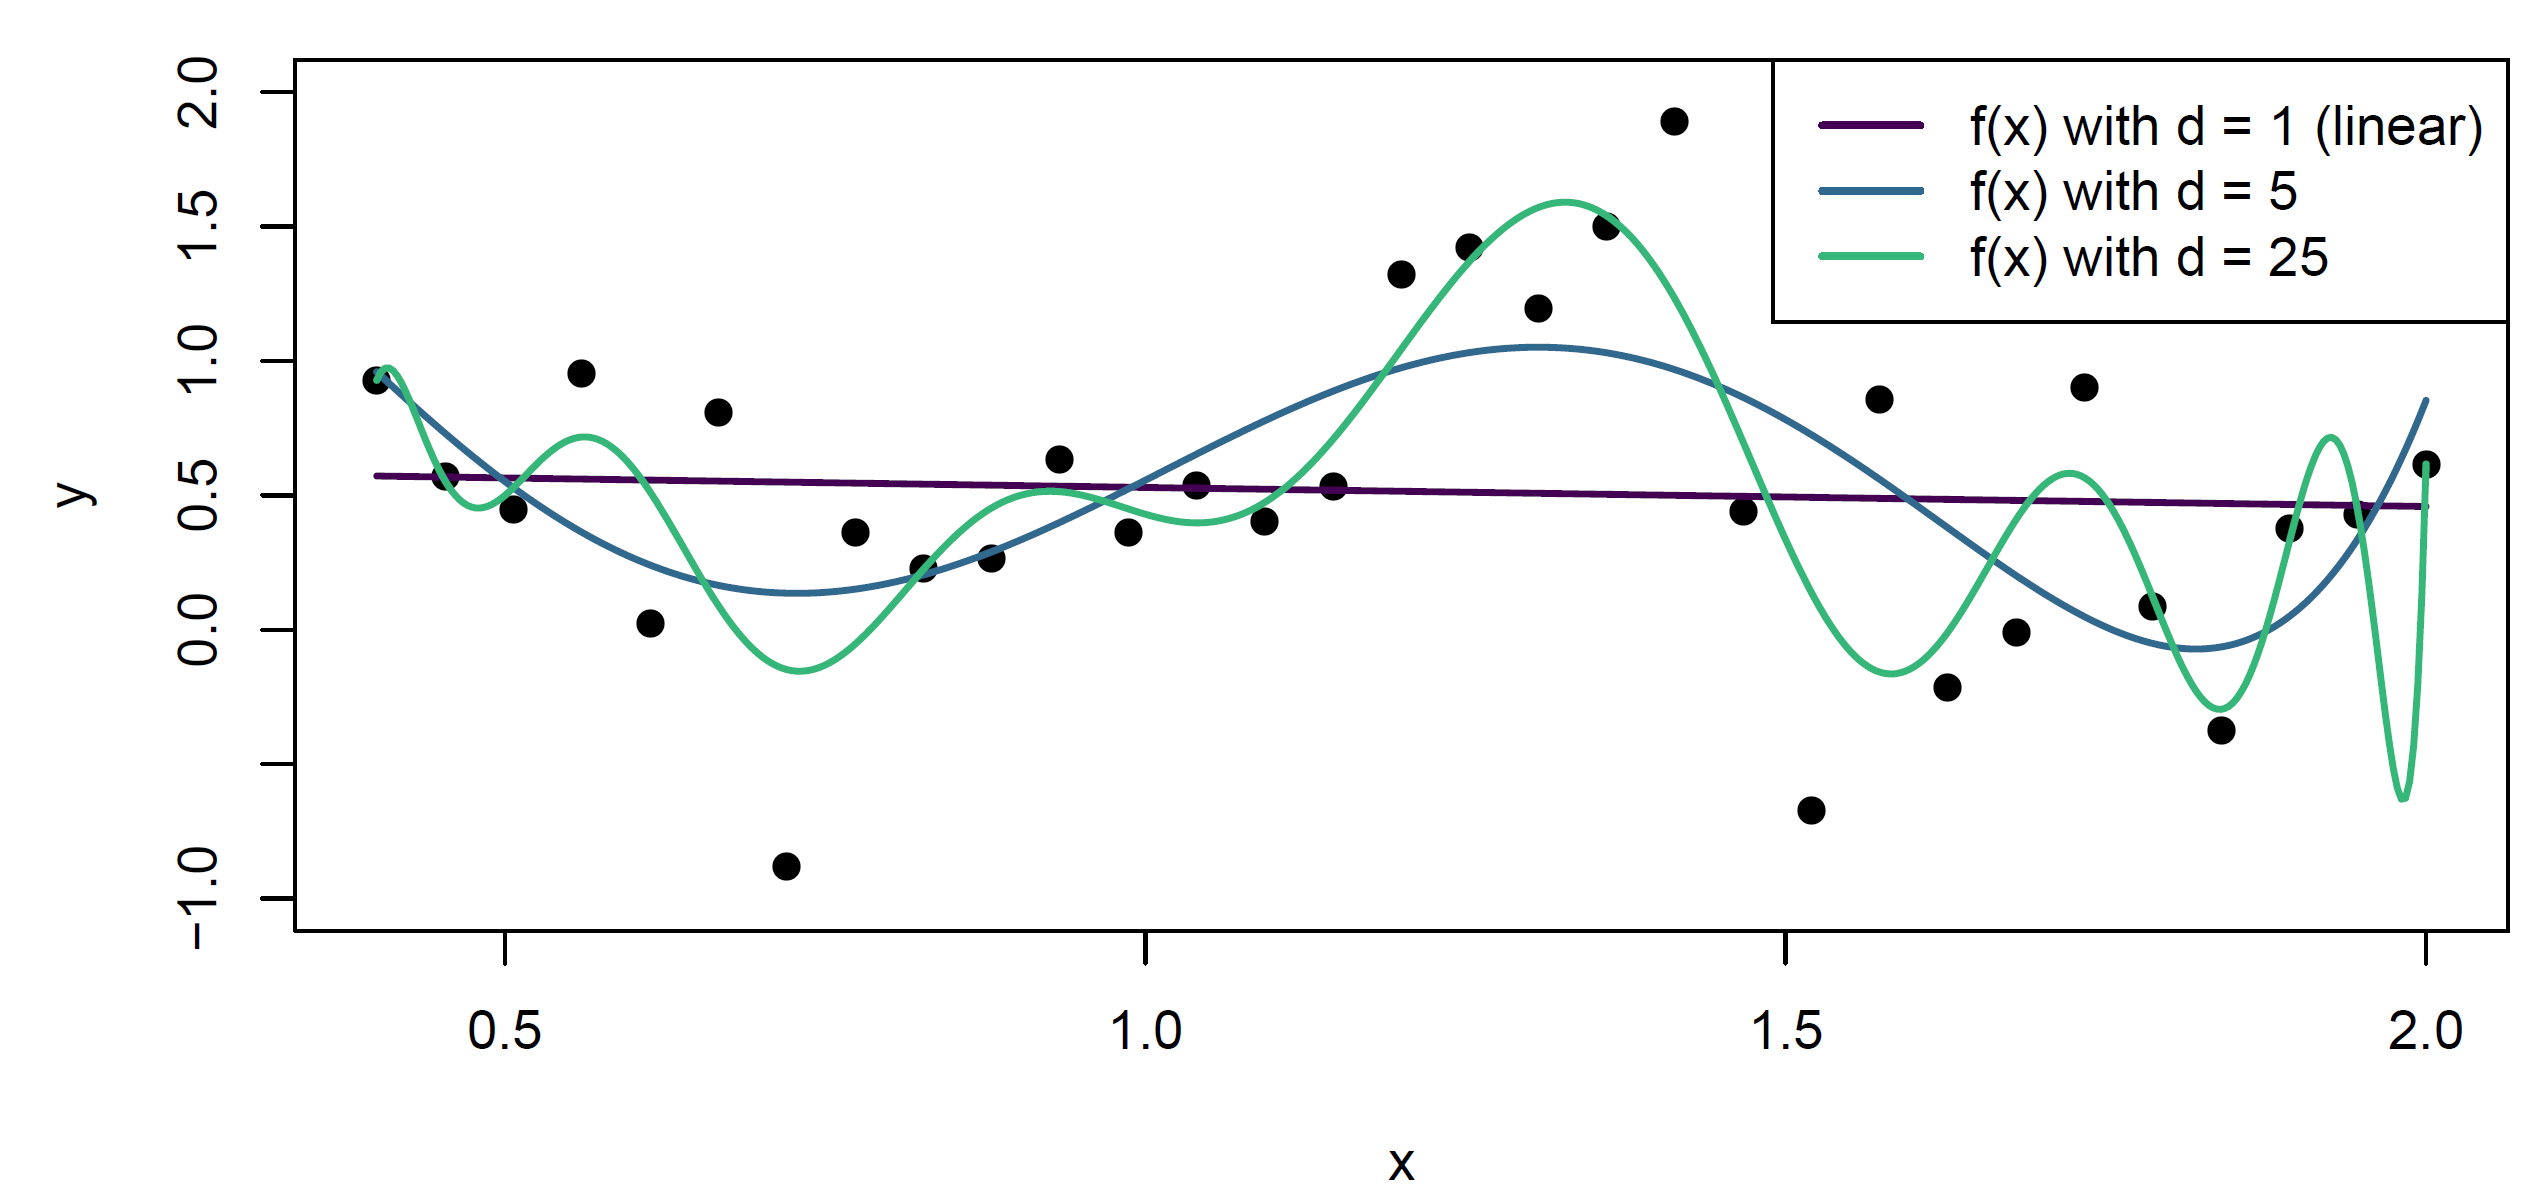
\includegraphics[width=0.91\columnwidth]{img/poly_reg.PNG}
  
  \end{myblock}
}
\end{minipage}
\end{beamercolorbox}
\end{column}
%%%%%%%%%%%%%%%%%%%%%%%%%%%%%%%%%%%%%%%%%%%%%%%%%%%%%%%%%%%%%%%%%%%%%%%%%%%%%%%%%%%%%
\begin{column}{.31\textwidth}
\begin{beamercolorbox}[center]{postercolumn}
\begin{minipage}{.98\textwidth}
\parbox[t][\columnheight]{\textwidth}{
  \begin{myblock}{ }
  The higher $d$ is, the more \textbf{capacity} the learner has to learn complicated functions of $x$, but
  this also increases the danger of \textbf{overfitting}
  
  \vspace*{1ex}
  
  \end{myblock}
  
  \begin{myblock}{K-Nearest Neighbors Regression}
  
  \textbf{K-NN} can be used for both regression and classification.
  \begin{codebox} \textbf{Basic Idea: }	\end{codebox}
  
  \begin{itemize}[$\bullet$]     
  \setlength{\itemindent}{+.3in}
    \item It generates predictions $\yh$ for a given $x$ by comparing the $k$ observations that are closest to $x$.
    \item "Closeness" requires a distance or similarity measure.
    \item The set containing the $k$ closest points $\xi$ to $x$ in the training data is called  the \textbf{k-neighborhood} $N_k(x)$ of $x$.
    \item $k$-NN makes no assumptions about the underlying data distribution.
    \item The smaller $k$, the less stable, less smooth and more \enquote{wiggly} the decision boundary becomes.
  \end{itemize}
  
  \begin{codebox}
  \textbf{Distance Measures: }
  \end{codebox}
  
  \begin{itemize}[$\bullet$]     
  \setlength{\itemindent}{+.3in}
  \item \textbf{The Euclidean distance}:
    \begin{equation*}
  d_{Euclidean}\left(x, \tilde{x}\right) = \sqrt{\sum_{j=1}^p(x_j- \tilde{x}_j)^2}
  \end{equation*}
  \item \textbf{Manhattan distance:}% based on the $L_1$-norm:
    \begin{equation*}
  d_{manhattan}(x, \tilde{x}) = \sum_{j=1}^p |x_j - \tilde{x}_j|
    \end{equation*}
  \item \textbf{Mahalanobis distance:} (takes covariances in $\mathcal{X}$ into account)
  
  \item
  \textbf{Gower distance:}
  $$d_{gower}(x,\tilde{x}) = \frac{\sum_{j=1}^p \delta_{x_j,\tilde{x}_j} \cdot d_{gower}(x_j,\tilde{x}_j)}{
    \sum_{j=1}^p \delta_{x_j,\tilde{x}_j}}.
  $$
    \end{itemize}
  
  \begin{codebox}
  \textbf{K-NN Summary: }
  \end{codebox}
  \textbf{Hypothesis Space:} Step functions over tesselations of $\Xspace$.
  Hyperparameters: distance measure $d(\cdot,\cdot)$ on $\mathcal X$; size of neighborhood $k$.
  
  \vspace*{1ex}
  
  \textbf{Risk:} Use any loss function for regression or classification.
  
  \vspace*{1ex}
  
  \textbf{Optimization:} Not applicable/necessary.
  
  \end{myblock}
}

\end{minipage}
\end{beamercolorbox}
\end{column}
\end{columns}
\end{frame}
\end{document}
